\chapter{Recolección y ordenamiento de información}
\section{Información materia prima para la investigación}


Para el proceso de investigación se tomo la población de los conjuntos residenciales de la constructora AR del barrio perdomo. La información fue recopilada por medio de la técnica de cuestionarios que fueron elaborados con la herramienta de formlarios de Google. 

La muestra para la investigación es de 129 personas encuestadas.

\section{Tabulación, ordenamiento y procesamiento de la información}

A continuación se presenta la información códificada:


\begin{table}
	\centering
	\begin{tabular}{|l|l|l|l|} 
		\hline
		\multicolumn{4}{|l|}{\textbf{CODIFICACIÓN}}                                                                                                                                                                                                                                       \\ 
		\hline
		\textbf{\begin{tabular}[c]{p{1cm}@{}l@{}} ITEM   \end{tabular}}                               & \textbf{PREGUNTA}                                                                                                                                                                          & \textbf{\centering \begin{tabular}[c]{p{1cm}@{}l@{}} SUB ITEM   \end{tabular}} & \textbf{\centering RESPUESTA}  \\ 
		\hline
		\multirow{2}{*}{1}                          & \multirow{2}{*}{\begin{tabular}[c]{p{9cm}@{}l@{}}¿El registro para el ingreso a la asamblea es organizado y rápido? \end{tabular}} & 1.1              & SI                  \\ 
		\cline{3-4}
		&                                                                                                                                                                                            & 1.2              & NO                  \\ 
		\hline
		\multirow{2}{*}{2~}                         & \multirow{2}{*}{\begin{tabular}[c]{p{9cm}@{}l@{}}La forma más efectiva de votación es: \end{tabular}}                                                                                        & 2.1              & PAPEL               \\ 
		\cline{3-4}
		&                                                                                                                                                                                            & 2.2              & ELECTRÓNICO         \\ 
		\hline
		\multirow{2}{*}{3}                          & \multirow{2}{*}{\begin{tabular}[c]{p{9cm}@{}l@{}}¿La presentación de los resultados de la Asamblea General es ágil y eficiente? \end{tabular}}                                                 & 3.1              & SI                  \\ 
		\cline{3-4}
		&                                                                                                                                                                                            & 3.2              & NO                  \\ 
		\hline
		\multirow{2}{*}{4}                          & \multirow{2}{*}{\begin{tabular}[c]{p{9cm}@{}l@{}}¿Actualmente cuenta con un celular Smartphone? \end{tabular}}                                                                                 & 4.1              & SI                  \\ 
		\cline{3-4}
		&                                                                                                                                                                                            & 4.2              & NO                  \\ 
		\hline
		\multirow{2}{*}{5}                          & \multirow{2}{*}{\begin{tabular}[c]{p{9cm}@{}l@{}}¿La duración de las Asambleas Generales es el adecuado? \end{tabular}}                                                                        & 5.1              & SI                  \\ 
		\cline{3-4}
		&                                                                                                                                                                                            & 5.2              & NO                  \\ 
		\hline
		\multirow{2}{*}{6}                          & \multirow{2}{*}{\begin{tabular}[c]{p{9cm}@{}l@{}}¿Cree que el conteo de los votos actualmente es confiable? \end{tabular}}                                                                     & 6.1              & SI                  \\ 
		\cline{3-4}
		&                                                                                                                                                                                            & 6.2              & NO                  \\ 
		\hline
		\multirow{2}{*}{7}                          & \multirow{2}{*}{\begin{tabular}[c]{p{9cm}@{}l@{}}¿Cree que una aplicación o sistema podría mejorar la efectividad de la asamblea? \end{tabular}}                                               & 7.1              & SI                  \\ 
		\cline{3-4}
		&                                                                                                                                                                                            & 7.2              & NO                  \\
		\hline
	\end{tabular}
\end{table}


\subsection{Ordenamiento}

Para el ordenamiento se presenta la cantidad de votos recibidos por cada una de las respuestas a continuación:


\begin{table}
	\centering
	\begin{tabular}{|l|l|l|l|} 
		\hline
		\multicolumn{4}{|l|}{\textbf{CODIFICACIÓN}}                                                                                                                                                                                                                                       \\ 
		\hline
		\textbf{\begin{tabular}[c]{p{1cm}@{}l@{}} ITEM   \end{tabular}}                               & 
		\textbf{\begin{tabular}[c]{p{1cm}@{}l@{}} SUB ITEM   \end{tabular}} & \textbf{RESPUESTA} & \textbf{TOTAL}  \\ 
		\hline
		\multirow{2}{*}{1} & 1.1 & SI & 8 \\ 
		\cline{3-4}  & 1.2 & NO & 121   \\ 
		\hline
		\multirow{2}{*}{2~} & 2.1  & PAPEL & 11 \\ 
		\cline{3-4} & 2.2  & ELECTRÓNICO & 118  \\ 
		\hline
		\multirow{2}{*}{3} & 3.1   & SI  & 8 \\ 
		\cline{3-4} &  3.2  & NO  & 121  \\ 
		\hline
		\multirow{2}{*}{4} & 4.1  & SI  & 118 \\ 
		\cline{3-4} & 4.2 & NO & 11 \\ 
		\hline
		\multirow{2}{*}{5} &  5.1 & SI & 6 \\ 
		\cline{3-4} & 5.2 & NO & 123 \\ 
		\hline
		\multirow{2}{*}{6}  & 6.1 & SI & 15 \\ 
		\cline{3-4}  & 6.2 & NO & 114 \\ 
		\hline
		\multirow{2}{*}{7} & 7.1 & SI & 120\\ 
		\cline{3-4} & 7.2 & NO & 9 \\
		\hline
	\end{tabular}
\end{table}

\subsection{Procesamiento}



\section{Presentación de resultados}

\subsection{Tablas}

\subsection{Histograma de distribución de frecuencia}

\subsection{Gráficos}

%%grafo

\begin{figure}[th!]
	\centering
	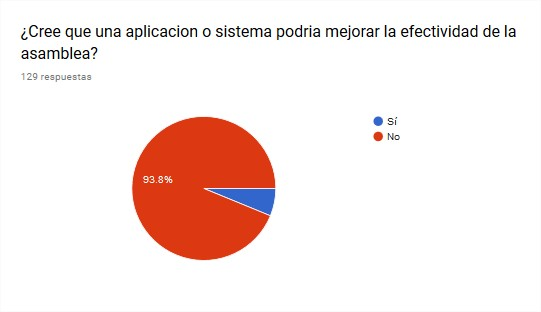
\includegraphics[width=0.7\linewidth]{desarrollo/resultados/imgs/pregunta-1}
	\caption{Gráfica pregunta 1}
\end{figure}

%%grafo

\begin{figure}[th!]
	\centering
	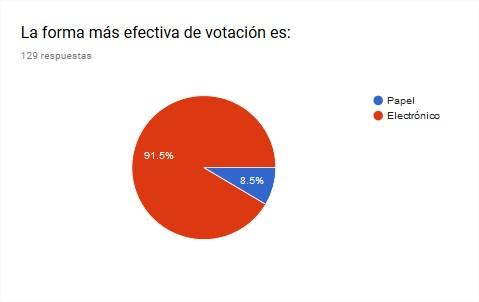
\includegraphics[width=0.7\linewidth]{desarrollo/resultados/imgs/pregunta-2}
	\caption{Gráfica pregunta 2}
\end{figure}

%%grafo

\begin{figure}[th!]
	\centering
	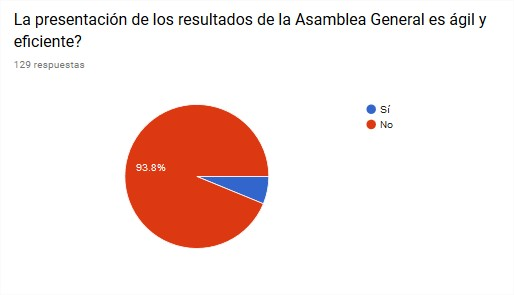
\includegraphics[width=0.7\linewidth]{desarrollo/resultados/imgs/pregunta-3}
	\caption{Gráfica pregunta 3}
\end{figure}

%%grafo

\begin{figure}[th!]
	\centering
	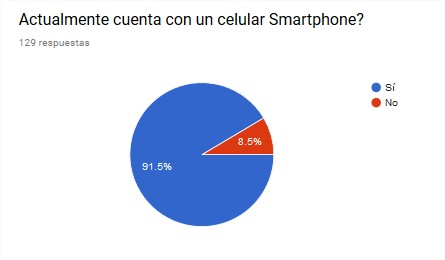
\includegraphics[width=0.7\linewidth]{desarrollo/resultados/imgs/pregunta-4}
	\caption{Gráfica pregunta 4}
\end{figure}

%%grafo

\begin{figure}[th!]
	\centering
	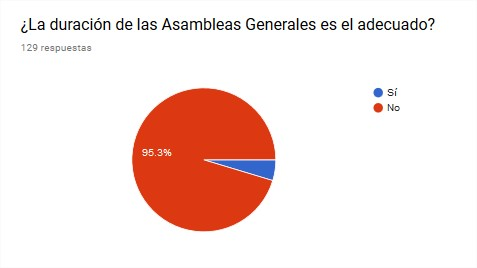
\includegraphics[width=0.7\linewidth]{desarrollo/resultados/imgs/pregunta-5}
	\caption{Gráfica pregunta 5}
\end{figure}

%%grafo

\begin{figure}[th!]
	\centering
	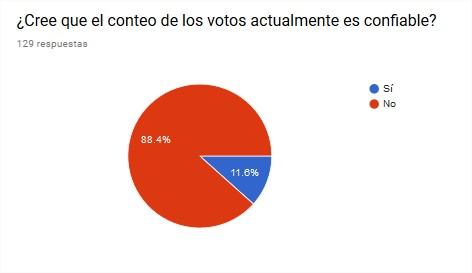
\includegraphics[width=0.7\linewidth]{desarrollo/resultados/imgs/pregunta-6}
	\caption{Gráfica pregunta 6}
\end{figure}

%%grafo

\begin{figure}[th!]
	\centering
	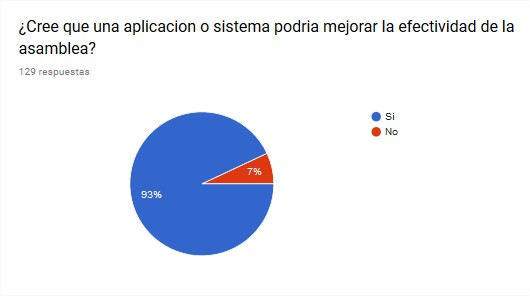
\includegraphics[width=0.7\linewidth]{desarrollo/resultados/imgs/pregunta-7}
	\caption{Gráfica pregunta 7}
\end{figure}


\newpage